\section{Metodologia}\label{sec-metodologia}

Não foi necessária uma análise ética prévia por parte dos conselhos de
projetos adequados para a investigação, uma vez que os participantes não
foram identificados. Por não haver conflito de interesses, a Texto Livre
não terá quaisquer consequências, inclusive assistência integral e
eventual, ressarcimento de qualquer dano resultante a qualquer dos
participantes da pesquisa, conforme a Resolução nº 510, de 7 de abril de
2016, do Conselho Nacional de Saúde do Brasil.

A metodologia é a explicação minuciosa, detalhada, rigorosa e exata de
toda a ação desenvolvida no método de trabalho da pesquisa \cite{lakatos2003}. A pesquisa é um estudo de caso, que teve o aluno como
objeto de estudo. \textcite[p. 32]{yin2005} argumenta que o estudo de caso visa a \enquote{conhecer em profundidade o como e o porquê de uma determinada
	situação que se supõe ser única em muitos aspectos, procurando descobrir
	o que há nela de mais essencial e característico}. O estudo de caso é
caracterizado pelo estudo profundo e exaustivo de um ou poucos objetos,
de maneira a permitir o seu conhecimento amplo e detalhado. O caso
experimental caracteriza-se por determinar um objeto de estudo,
selecionar as variáveis que seriam capazes de influenciá-lo, definir as
formas de controle e de observação dos efeitos que a variável produz no
objeto \cite{gil2002}. A coleta dos dados foi realizada em uma escola
secundária do sul de Moçambique. Fizeram parte da amostra 50 alunos do
ensino secundário, selecionados de forma aleatória, dos quais 25
participaram do estudo das PO e aplicação do Q3DM. Os restantes 25
estiveram envolvidos no estudo das SCs e aplicação do GeoGebra. Em ambos
os estudos, todos os alunos experimentaram as aplicações (Q3DM ou
GeoGebra). A pesquisa apresenta um estudo de caso interpretativo, o qual
desenvolve categorias conceituais indutivamente para examinar os
pressupostos iniciais, as intenções e significados das ações e
expressões dos alunos \cite{amado2017}. A compreensão interpretativa é
sustentada a partir do relato pormenorizado da interação dos sujeitos em
seu meio natural \cite{coulon1995}. A visão interpretativa descreveu as
ações dos alunos em ambiente de sala de aula e os significados das ações
no processo de toda a pesquisa \cite{coutinho2011}.

Foi possível, pois, observar e interpretar tudo o que ocorreu, tornando
viável a análise das relações causa-efeito. Foi possível , também,
qualificar as ações dos alunos em todo o processo de aprendizagem, por
meio das interpretações dos significados de seus comportamentos durante
a mediação da aula e as respostas do questionário de satisfação. Além
disso, os dados foram coletados por meio das técnicas de observação do
participante, com tomada de notas e de registro fotográfico, assim como
dos instrumentos de coleta de dados aplicados, como os questionários de
satisfação.

\subsection{Realização das aulas}\label{sub-sec-Realização das aulas}

As aulas consistiram na apresentação de dois temas, PO e SCs, de forma
separada. Para os alunos da 9ª classe, o tema de pesquisa foi PO, e foi
utilizado o Q3DM. A professora primeiramente apresentou o tema,
explicando o que eram POs, dizendo que eram figuras geométricas sobre um
plano que poderiam ser comparadas à sombra do mesmo objeto no horário em
que o sol estaria no ponto mais alto no dia. Depois, demonstrou as
vistas ortogonais do sólido. (Ver \Cref{fig-03}).

\begin{figure}[htpb]
\centering
\begin{minipage}{.5\textwidth}
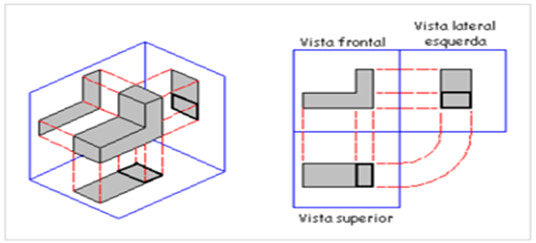
\includegraphics[width=\textwidth]{figures/figure03.jpg}
\caption{Vistas ortogonais e ortográficas: vista frontal; vista superior; e vista lateral esquerda.}
\label{fig-03}
\source{\url{http://turmag1215vialonga.blogspot.com/2014/10/projecoes-ortogonais.html}.}
\end{minipage}
\end{figure}

Posteriormente a professora apresentou a aplicabilidade das POs, dizendo
que eram destinadas à planificação de vários objetos. Com o auxílio das
simulações computacionais, construiu os sólidos geométricos e demonstrou
suas vistas ortogonais, apresentando os procedimentos para a manipulação
do Q3DM. (Ver \Cref{fig-04})

\begin{figure}[htpb]
\centering
\begin{minipage}{.5\textwidth}
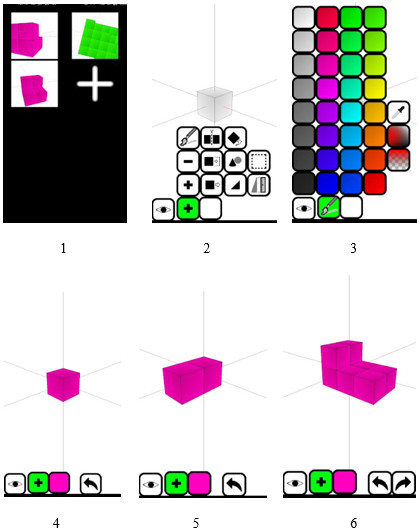
\includegraphics[width=\textwidth]{figures/figure04.jpg}
\caption{Manipulação no Q3DM.}
\label{fig-04}
\source{Elaboração própria.}	
\end{minipage}
\end{figure}


A manipulação no Q3DM é feita por meio de cubos chamados Qubes, que
facilitam a criação e a montagem de objetos em três dimensões,
utilizando elementos digitais que podem ser inseridos, removidos,
deslocados, ampliados, inclinados, moldados geometricamente, girados e
coloridos.

Para os alunos da 12ª classe, o tema de pesquisa foi SCs e foi utilizado
o GeoGebra. A professora iniciou com a apresentação do tema SCs de
cilindro, explicando que a seção cilíndrica é uma figura resultante de
um plano secante no cilindro. A professora acrescentou que existem duas
situações distintas: quando o plano secante é paralelo ao eixo central
do cilindro; e quando o plano secante não é paralelo ao eixo central do
cilindro (ver as figuras \Cref{fig-05} e \Cref{fig-06}).

\begin{figure}[htpb]
\centering
\begin{minipage}{.25\textwidth}
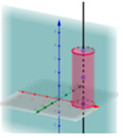
\includegraphics[width=\textwidth]{figures/figure05.jpg}
\caption{Secção paralela ao eixo central do cilindro.}
\label{fig-05}
\source{Elaboração própria.}
\end{minipage}
\end{figure}

\begin{figure}[htpb]
\centering
\begin{minipage}{.5\textwidth}
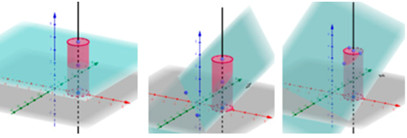
\includegraphics[width=\textwidth]{figures/figure06.jpg}
\caption{Secção não paralela ao eixo central do cilindro.}
\label{fig-06}
\source{Elaboração própria.}
\end{minipage}
\end{figure}

A professora, primeiramente, apresentou os diferentes posicionamentos
dos planos em relação ao eixo central do cilindro. Em seguida, com o
auxílio da tecnologia, apresentou à turma o software de geometria
dinâmica GeoGebra, indicando as funcionalidades de suas ferramentas e
como construir do ponto até o plano secante, com a ajuda dos
procedimentos para a sua manipulação no GeoGebra. Os alunos simularam as
SCs com o plano de nível; eles apresentaram-se atentos e motivados em
aprender a resolver o exercício no GeoGebra, particularmente para os
rapazes, os quais procuravam descobrir como construir diferentes sólidos
geométricos e como simular as VOs (vistas ortogonais).

\subsection{Realização do questionário}\label{sub-sec-Realização do questionário}

O questionário de satisfação aplicado teve como objetivo compreender se
o Q3DM e o GeoGebra facilitaram a aprendizagem das POs e SCs, e se o
\textit{smartphone} foi fácil de manipular. Ambos os questionários foram
preenchidos em 10 minutos. As questões visavam a coletar, nos dois
estudos, várias opiniões, incluindo: (1) se os aplicativos tecnológicos
facilitaram as representações 3D; (2) qual é a opinião deles sobre os
benefícios de usar os aplicativos ou se seria melhor resolver de forma
tradicional; (3) se os aplicativos são fáceis e intuitivos de usar; (4)
quais foram os aspectos positivos e negativos da aula; e, (5) como eles
classificariam a aprendizagem com o auxílio dos aplicativos.
